\documentclass[12pt,letterpaper]{report}
\usepackage[margin=1in]{geometry}
\usepackage{titlesec}
\usepackage{amsmath}
\usepackage{amssymb}
\usepackage[colorlinks=true,urlcolor=black,linkcolor=black]{hyperref}
\usepackage{graphicx}
\usepackage{textcomp}
% extra packages you need

\titleformat{\chapter}{\bf\huge}{\thechapter}{20pt}{\huge\vspace{-.5em}}

\begin{document}
\title{Software Measurement (SOEN6611)\\[.5em]
Summer 2023\\[.5em]
Descriptive Statistics\\[.5em]
Team "Amsterdam Cartel"\\[.5em]
Deliverable 1}
\author{Unnati Chaturvedi, Mengqi Liu, Lei Zhou, Hema Reddy Mupppidi}
\maketitle

\pagenumbering{roman}
\setcounter{page}{0}

\tableofcontents

\chapter*{List of Symbols and Abbreviations}\addcontentsline{toc}{chapter}{List of Symbols and Abbreviations}



% delete these example entries
\noindent\begin{tabular}{ll}
% $\mathbb{R}$ & The set of real numbers (example)\\
% $\|\cdot\|_F$ & Frobenius norm (example)\\
GQM & Goal Question Metric\\
UC & Use Case

\end{tabular}

% delete this section if no figures
\listoffigures\addcontentsline{toc}{chapter}{List of Figures}
% This will automatically be populated if you included figures in your report.


%%%%%%%%%%%%%%%%%%%%%%%%%%%%%%
\chapter{Introduction}
\pagenumbering{arabic}

\section{Problem 1}

% delete this text
Using the Goal-Question-Metric (GQM) approach (or one of its extensions), present one goal specific to METRICSTICS and articulte 2N questions related to that goal, where N is the team size. Discuss whether any metrics help answer those questions. NOTES: The goals must aim to be SMART. 
					
There are four phases in the GQM measurement process: 
(1) Planning Phase,
(2) Definition Phase, 
(3) Data Collection Phase, and 
(4) Interpretation Phase

\begin{figure}[h]
    \begin{center}
    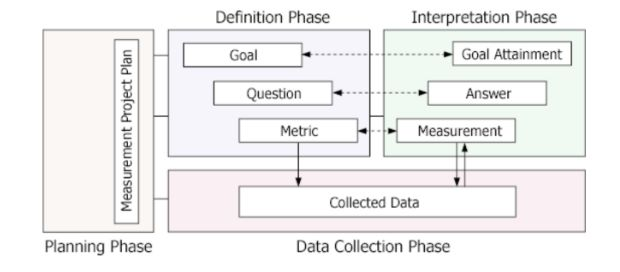
\includegraphics[width=0.8\linewidth]{1.jpg}
    \end{center}
       \caption{Data Planning and Collection Phase \label{Data Planning and Collection Phase}}
\end{figure}


\subsection{Smart}
The goal is considered to be smart if it has the following qualities:

\textbf{ Specific}: Is the goal specific? (For example, is the goal too general to be understandable?) 	

\textbf{Measurable}: Is the goal associated with quantitative criteria for verifying attainment?

\textbf{Attainable}: Is there a consensus that this goal is achievable? (For example, is the goal too impractical to be feasible?) Is there resource allocation towards the goal?

\textbf{Realistic}: Is the goal rationalized? (For example, is it clear why an entity is being measured?) Is the goal within the scope of what the person responsible for software measurement program is expected to accomplish?

\textbf{Timely}: Is the goal time-limited (that is, is there a specific start- and end-date for the goal)? (For example, is there time allocated in the project schedule toward collecting data and tracking progress toward the goal?) 


\section{Problem 2}

% delete this text

Using the given description, construct a use case model for METRICSTICS. This description must include definitions of actors and use cases. NOTES There can be several use cases, including saving data in memory, restarting a session, and so on. A statistical calculator1 could be used as a motivation to ‘elicit’ necessary use cases. 

\begin{figure}[h]
    \begin{center}
    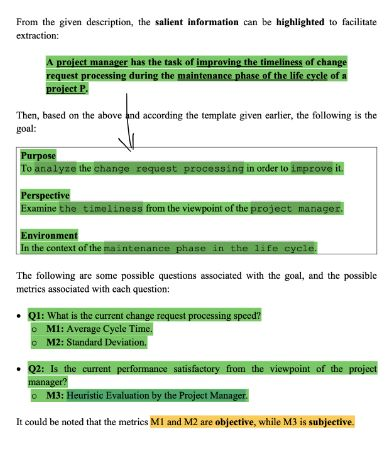
\includegraphics[width=0.8\linewidth]{2.jpg}
    \end{center}
\end{figure}


\section{dataset}

https://www.kaggle.com/code/knightbearr/analysis-sales-data-knightbearr/input?select=Sales December 2019.csv


%%%%%%%%%%%%%%%%%%%%%%%%%%%%%%
\chapter{Problem 1}

\section{Goal}

To develop the Sales Analytics System, named METRICSTICS, a critical system will be implemented in order to comprehensively analyze sales performance. This subsystem will seamlessly integrate with the in-store sales system, facilitating the collection of detailed customer data.\\[1\baselineskip]

This system will examine statistical analysis of sales data to empower the sales management team in effectively monitoring sales trends over time, conducting thorough analyses of sales history, and making informed decisions based on the insights gained. Both sales staff and sales administration personnel will have access to METRICSTICS, allowing the sales team to diligently input sales data and the sales manager to effortlessly access statistical information for specific time periods. Additionally, METRICSTICS will enable the generation of comprehensive reports on a monthly, quarterly, and yearly basis, which will be presented to the board of members.		 	 	 	

*Note: The key stakeholders for METRICSTICS are sales representatives, sales managers


\section{Analyze Metricstics}

% delete this text

Analyze the sale's history to understand the sale trend during the years to project METRICSTICS from the viewpoint of the sales manager


1. What is the percentage increase or decrease in sales over each month?
Metric: Calucate\\[1\baselineskip]

2. What is the average of sales monthly and quarterly? (Mean)
Metric: 
Average(Mean) monthly sales
Average(Mean) quarterly sales
Mechanism:
i. Owner = Sales Managers
ii. Frequency Collected = following the monthly report generation
iii. Frequency Reported = Monthly and Quarterly\\[1\baselineskip]

3. What is the biggest sales growth and decline rate this year by monthly and quarterly? (MAX and MIN)
metric:
Maximum monthly sales decline rate
Minimum monthly sales decline rate
Maximum quarterly sales decline rate
Minimum quarterly sales decline rate
Mechanism:
i. Owner = Sales Managers
ii. Frequency Collected = following the monthly report generation
iii. Frequency Reported = Monthly and Quarterly\\[1\baselineskip]


4. How to determine that each month's and quarter’s  sales experience growth or decline?
Metric: compute the baseline(MAD) in terms of monthly and quarterly sale, and compare it in monthly sale and quarterly sale.
Mechanism:
i. Owner = Sales Managers
ii. Frequency Collected = following the monthly report generation
iii. Frequency Reported = Monthly and Quarterly\\[1\baselineskip]

5. Which month and quarter experienced the most significant sales change over the year? (standard deviation)(mean)
Metric: standard deviation of monthly and quarterly sales
Mechanism:
i. Owner = Sales Managers
ii. Frequency Collected = following the monthly report generation
iii. Frequency Reported = Monthly and Quarterly\\[1\baselineskip]


6. Question(Mode): How to calculate the top 10 items that customers purchased at least twice on this platform monthly and quarterly, sorted by the number of purchases 
Metric: Count the number of times each item is purchased in a month, find the items purchased more than once and sort them by their purchasing times, both in monthly and quarterly.
Mechanism:
i. Owner = Sales Managers
ii. Frequency Collected = following the monthly and quarterly report generation
iii. Frequency Reported = monthly and quarterly\\[1\baselineskip]


7. Question (Mode): What is the most popular item monthly?
Metric: Count the number of times each item is purchased in a month and find the item with the highest count.
Mechanism:
i. Owner = Sales Managers
ii. Frequency Collected = following the monthly report generation
iii. Frequency Reported = Monthly\\[1\baselineskip]


8. Question(Mode): In which city residents make the biggest purchases on this platform for the whole year?
Metric: Count the number of purchases based on the city extracted from purchase addresses and find the city with the highest count.
Mechanism:
i. Owner: Sales Managers
ii. Frequency Collected = following the yearly report generation
iii. Frequency Reported = Yearly\\[1\baselineskip]


9. Question (Max): How to determine the day of the year when people engage in the highest amount of shopping?
Metric: Count the number of purchases each day in a year and find the day with the highest count.
Mechanism:
i. Owner = Sales Managers
ii. Frequency Collected = following the yearly report generation
iii. Frequency Reported = Yearly\\[1\baselineskip]


%%%%%%%%%%%%%%%%%%%%%%%%%%%%%%
\chapter {Problem 2}

\section{Use Case Model}

\begin{figure}[h]
    \begin{center}
    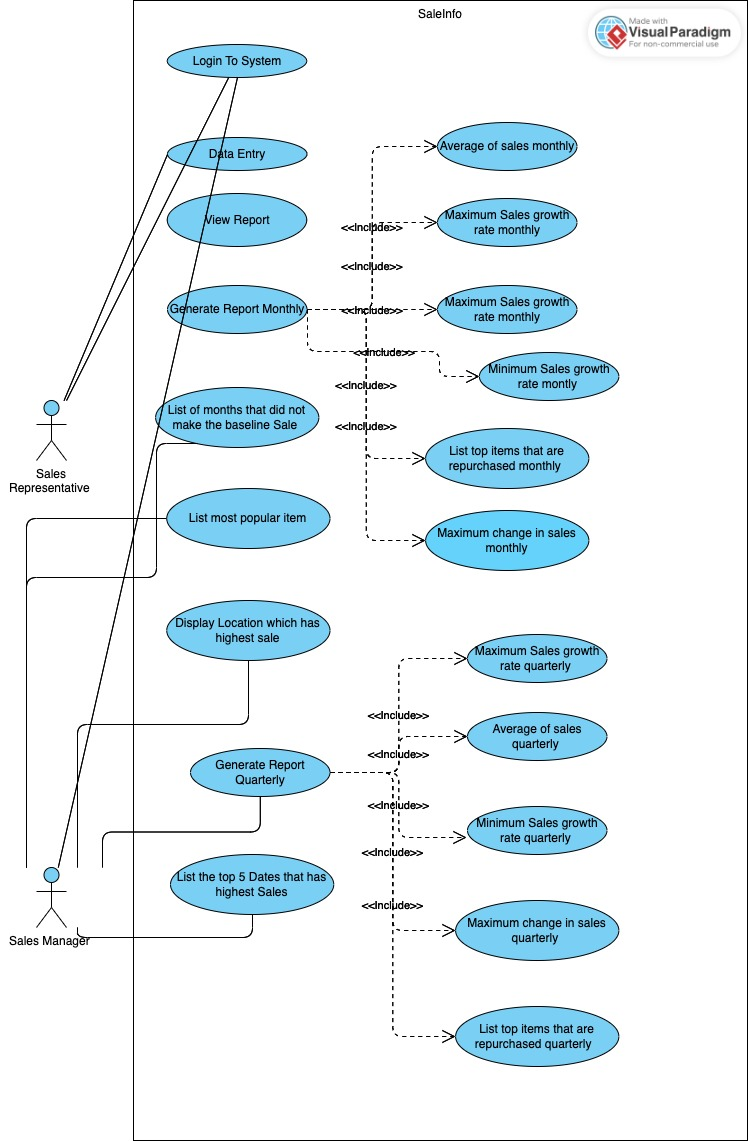
\includegraphics[width=0.8\linewidth]{14.jpg}
    \end{center}
       \caption{Use Case Model \label{Use Case Model}}
\end{figure}

\underline{Login in to the system}\\
Primary Actor: Sale Representative, Sale Manager\\
Prioity: High\\
Description:Users are able to login to the system\\
Pre-condition: User have valid account on the system\\
Normal Flow: \\
User open the login page of the system\\
System display the login page\\
User enter username and password\\
User Clicks on “login” button\\
System check the User’s credentials\\
System display the home page\\
User see the home page.\\[1\baselineskip] \underline{Sale staffs are able to do the data entry}\\
Primary Actor: Sale Representative\\
Prioity: High\\
Description:Sale Representatives are able to entry the data regarding the customer purchasing item\\
Pre-condition: Sale Representative login to the system\\
Normal Flow: \\
User able to see the data entry page\\
System display the data entry page\\
Users are able to enter the name of the item, purchase date, customer’s address, quantity of item, and etc.\\
User click the submit button\\
System store the sale data to database\\
System redirect to data entry page again with empty input.\\[1\baselineskip] \underline{Sales managers are able to view the statistics result generated from the sales history data}\\
Primary Actor: Sales Manager\\
Prioity: High\\
Description:Sales Manager is able to view the statistics result generated from the sales history data\\
Pre-condition: Sales Manager is able to login to the system.\\ Corresponding sales data are ready in the system.\\
Normal Flow: \\
User is able to see the report page\\
User is able to enter the conditions for the report, like time duration or specific month, etc.\\
User clicks the submit button to calculate the statistics\\
User is able to view the statistics results.\\[1\baselineskip] \underline{Generate report in monthly and quarterly}\\
Primary Actor: System itself or Sales Manager\\
Prioity: High\\
Description:Sales Manager is able to generate the statistics report in both monthly and quarterly\\
Pre-condition: Sales Manager is able to login to the system. Sales data is ready in the system.\\
Normal Flow:\\
User is able to see the report page\\
User is able to enter the conditions for the report, like time duration or specific month, etc.\\
Or sales manager sets the needed report and the system itself will generate on time.\\[1\baselineskip] \underline{Other Possible Use Cases ??}\\
Sale manager are able to see the average sale in monthly\\
Display month-over-month ratio\\
Display current status of sale pass the baseline or not\\
Display 10 popular item based on past sale history\\
Display popular item in monthly\\

\begin{figure}[h]
    \begin{center}
    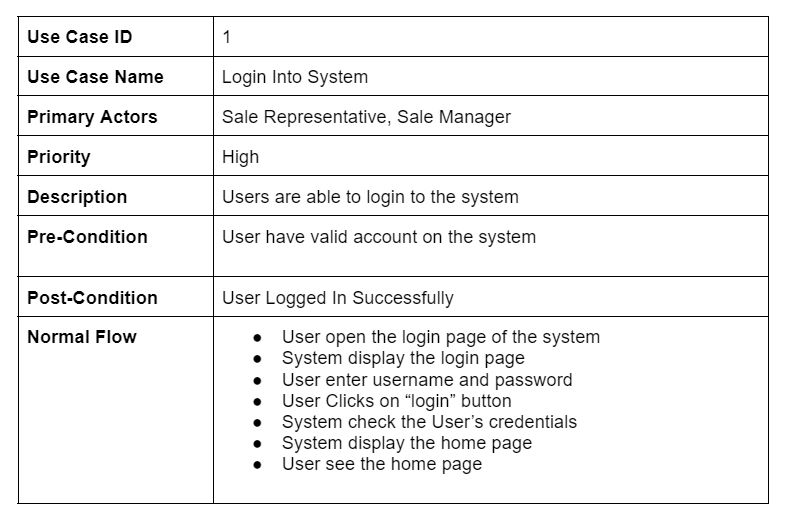
\includegraphics[width=0.8\linewidth]{4.jpg}
    \end{center}
       \caption{Use Case 1 \label{Use Case 1}}
\end{figure}

\begin{figure}[h]
    \begin{center}
    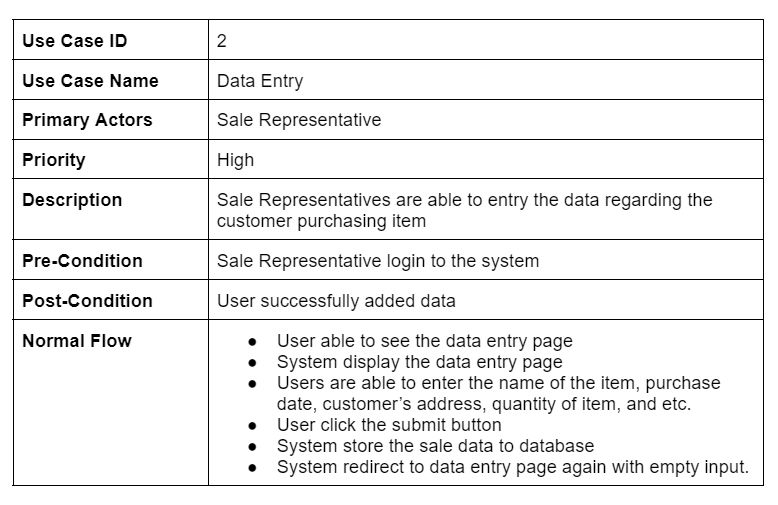
\includegraphics[width=0.8\linewidth]{5.jpg}
    \end{center}
       \caption{Use Case 2 \label{Use Case 2}}
\end{figure}

\begin{figure}[h]
    \begin{center}
    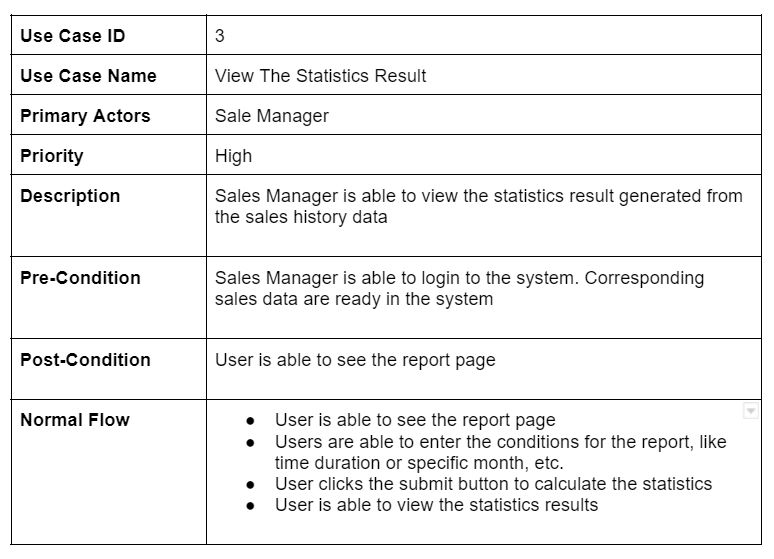
\includegraphics[width=0.8\linewidth]{6.jpg}
    \end{center}
       \caption{Use Case 3 \label{Use Case 3}}
\end{figure}

\begin{figure}[h]
    \begin{center}
    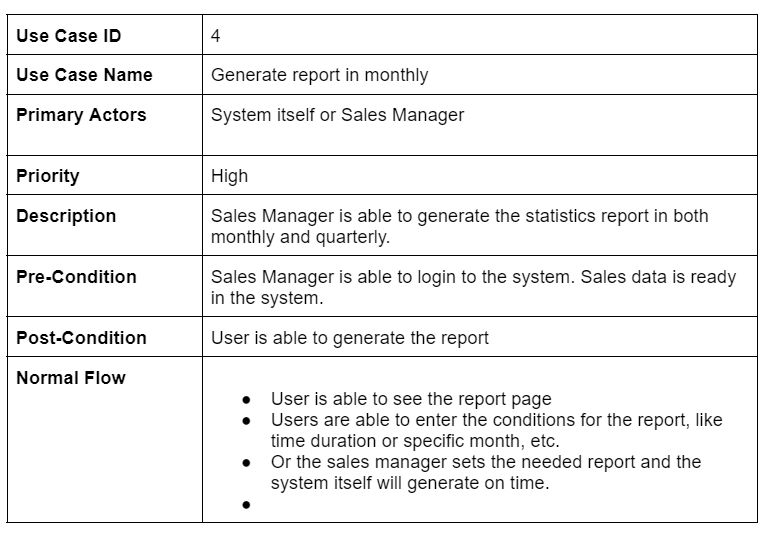
\includegraphics[width=0.8\linewidth]{7.jpg}
    \end{center}
       \caption{Use Case 4 \label{Use Case 4}}
\end{figure}

\begin{figure}[h]
    \begin{center}
    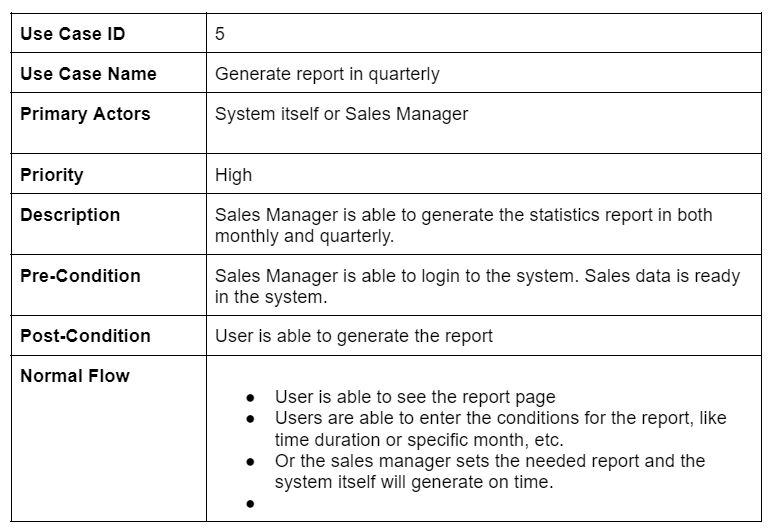
\includegraphics[width=0.8\linewidth]{8.jpg}
    \end{center}
       \caption{Use Case 5 \label{Use Case 5}}
\end{figure}

\begin{figure}[h]
    \begin{center}
    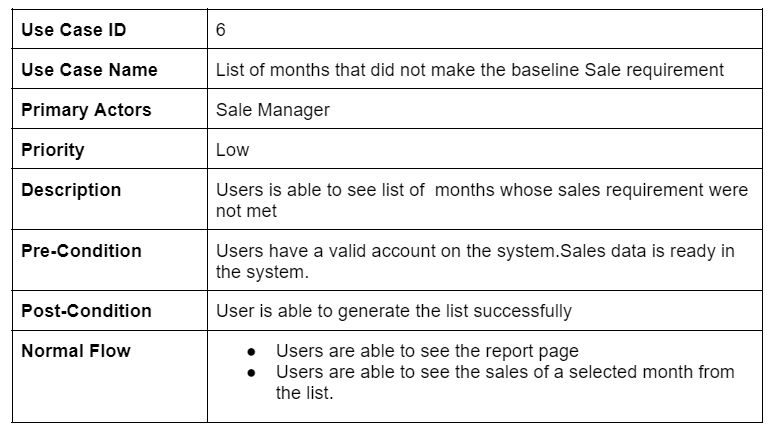
\includegraphics[width=0.8\linewidth]{9.jpg}
    \end{center}
       \caption{Use Case 6 \label{Use Case 6}}
\end{figure}

\begin{figure}[h]
    \begin{center}
    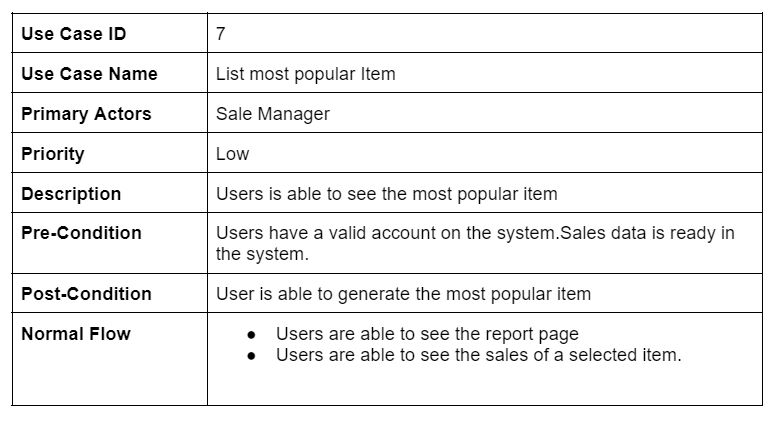
\includegraphics[width=0.8\linewidth]{10.jpg}
    \end{center}
       \caption{Use Case 7 \label{Use Case 7}}
\end{figure}

\begin{figure}[h]
    \begin{center}
    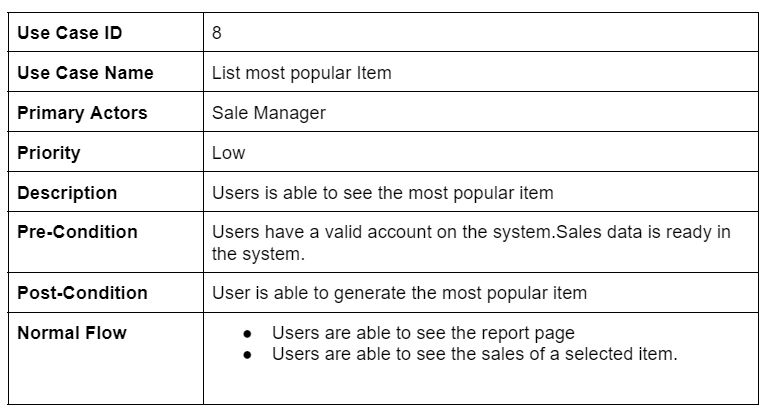
\includegraphics[width=0.8\linewidth]{11.jpg}
    \end{center}
       \caption{Use Case 8 \label{Use Case 8}}
\end{figure}

\begin{figure}[h]
    \begin{center}
    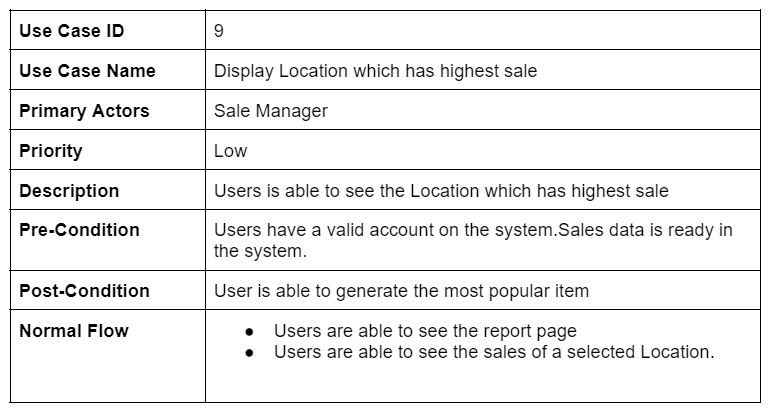
\includegraphics[width=0.8\linewidth]{12.jpg}
    \end{center}
       \caption{Use Case 9 \label{Use Case 9}}
\end{figure}

\begin{figure}[h]
    \begin{center}
    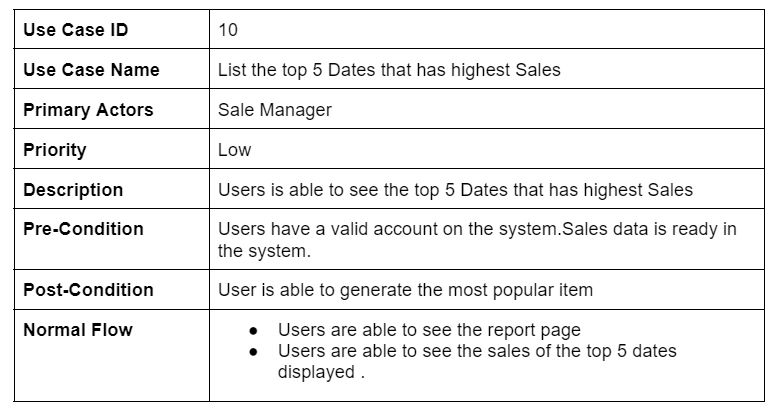
\includegraphics[width=0.8\linewidth]{13.jpg}
    \end{center}
       \caption{Use Case 10 \label{Use Case 10}}
\end{figure}


\section{Github Repository}

https://github.com/hemareddy123/SOEN\_6611\_Summer2023/tree/main


%%%%%%%%%%%%%%%%%%%%%%%%%%%%%%

\begin{thebibliography}{7}
    \addcontentsline{toc}{chapter}{Bibliography}

    % delete all of these example references, and replace them with references for your report.
    
    \bibitem{Lecture Slides} 
    Lecture Slides 
    \textit{Lecture slides"SOEN6611 Course Website”}.     
    
     \bibitem{Software Measurement Metrics} 
    Metrics.,
    \\\texttt{https://www.geeksforgeeks.org/software-measurement-and-metrics/}
    
    \bibitem{Use Case Diagram} 
    Use Case Diagram.,
    \\\texttt{https://www.visual-paradigm.com/guide/uml-unified-modeling-language/what is use case diagram/}

 
    

    
\end{thebibliography}



\end{document}
